\begin{frame}{Vectorization}
	Requirements:
	\begin{itemize}
		\item No loop carried dependency
		\item Loop bounds
		\item No jumps in code
	\end{itemize}
	
	Realising it:
	\begin{itemize}
		\item \#pragma omp simd
		\item Compiling with -O3
		\item Using Intel Icx Compiler
	\end{itemize}
\end{frame} 

\begin{frame}{Vectorization - Results MP-Media}
	\note{
		\begin{itemize}
			\item Difference: Annotation of simd to loop
			\item Both compiled with -O3
			\item Possibly auto vectorization
			\item ICX much worse for MP-Media
			\item SIMD more stable
		\end{itemize}	
	}
	\centering
	\vspace{-5pt}
	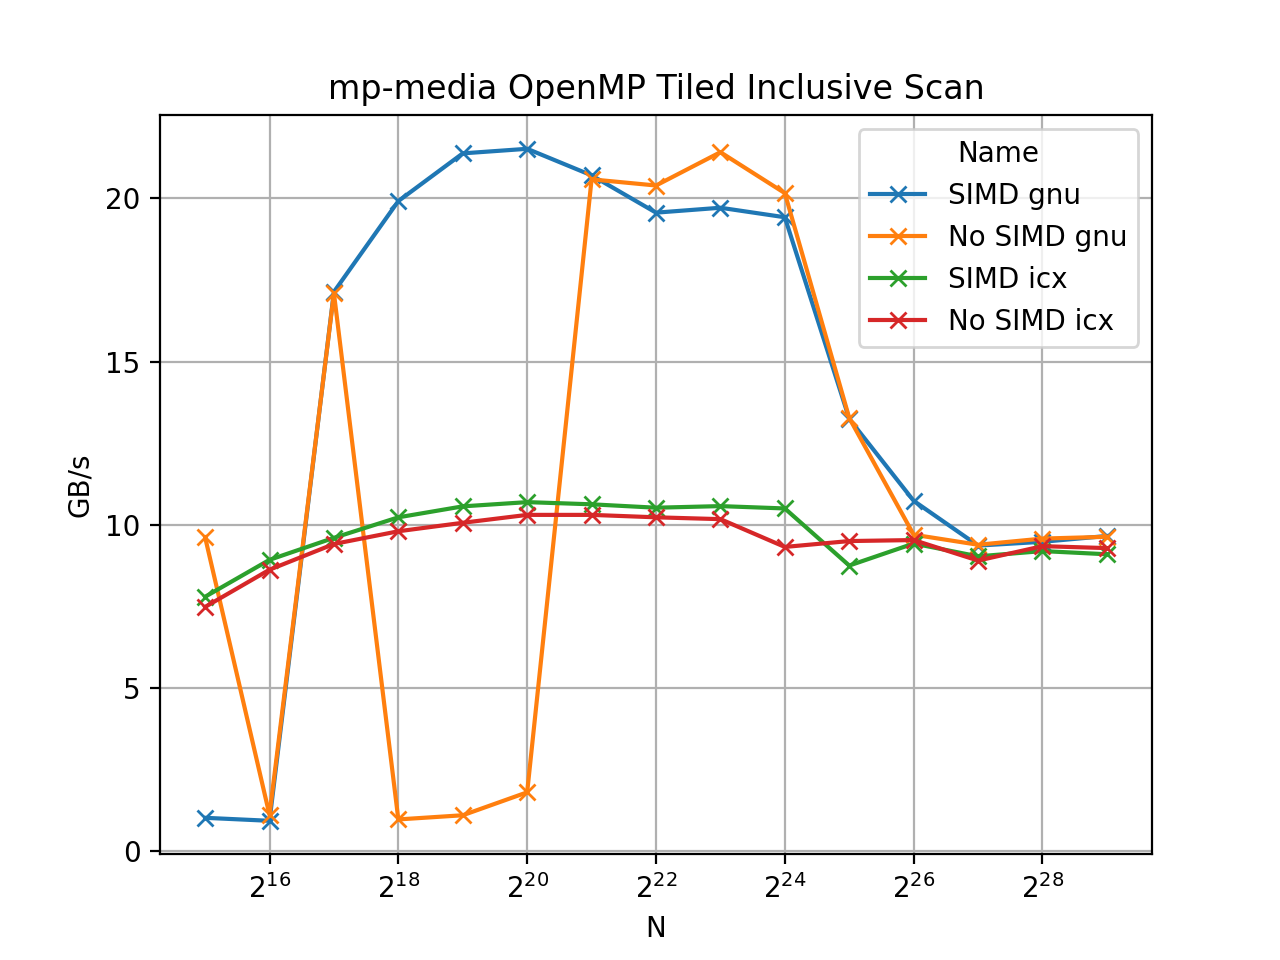
\includegraphics[width=0.90\textwidth]{graphs/mp-media OpenMP Tiled Inclusive Scan.png}
\end{frame}

\begin{frame}{Vectorization - Results Ziti-Rome}
	\note{
		\begin{itemize}
			\item Possibly auto vectorization
			\item ICX much better for ziti-rome
			\item SIMD better performance
			\item => SIMD
		\end{itemize}	
	}
	\centering
	\vspace{-5pt}
	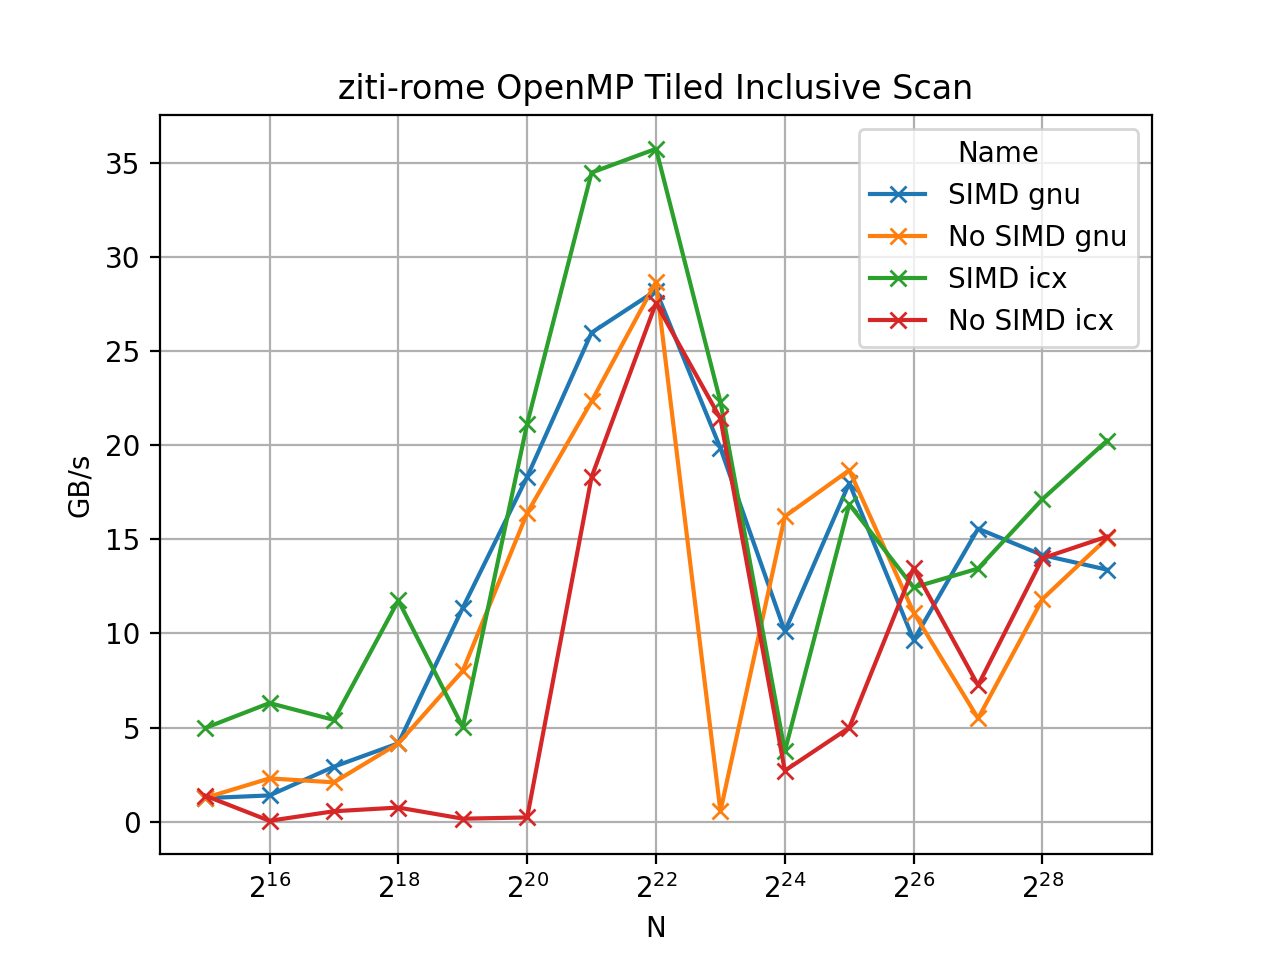
\includegraphics[width=0.90\textwidth]{graphs/ziti-rome OpenMP Tiled Inclusive Scan.png}
\end{frame}
